\setchapterpreamble[u]{\margintoc}
\chapter{The traceability matrices}
\label{sec:TraceabilityMatrices}

In a customer request for proposal, the need is usually given through a list of requirements. The supplier sends back a proposal showing his solution through a list of specifications. The coverage between requirements and specifications can take different shapes:

\begin{itemize}
    \item 1 to 1: one specification covers one requirement
    \item 1 to many: several specifications are used to cover only one requirement
    \item Many to 1: several requirements are covered by one specification.
\end{itemize}

But in practice, it is rather a mix of the three leading to a maze of coverage. Fortunately the traceability matrix shows up to bring some order.


\section{Traceability, this entangled mess}
A document size can vary a lot depending on the different fields of activity it deals with. To explain this, I will take an example I know well. Consider a request for proposal (RFQ) about an aeronautic calculator. Please don’t leave yet! I’ll make it clear.

In a plane, there are dozens of calculators. Those are computers without a screen or a keyboard. They manage everything, from the air conditioning to the brakes, the doors, the electrical power distribution, etc. Whether their tasks are complex or very complex, their request for proposal can easily reach a hundred pages and hundreds of requirements. Several expertises are involved to describe all the requirements. For example:

\begin{itemize}
    \item electronics for the circuit boards
    \item mechanics for the case housing the circuit boards
    \item developers for the embedded firmware of the circuit boards
    \item etc.
\end{itemize}
Then this RFQ is sent to a supplier. He will study it with his teams to build the specifications. Sometimes several requirements can be covered by the same specification.

\subsection{Many to one}
Customer requirement 1: the circuit board shall be hermetically protected\\
Customer requirement 2: the case shall have the following measurements : X, Y, Z

Supplier specification 1: the case shall be from the brand B and the model M

Therefore the supplier specification hits two birds with one stone because the chosen case matches both the requirements.

\begin{figure}[h]
    \centering
    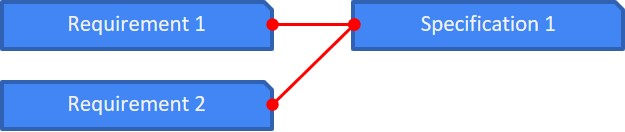
\includegraphics[]{ManyToOne.jpg}
    \caption{2 requirements covered by 1 specification}
    \label{fig:ManyToOne}
\end{figure}

\subsection{One to many}
But sometimes, it is the other way around! The requirement is so complex, it requires several specification to be fully covered:

Customer requirement 3: the circuit board shall be fully operational while the plane is flying (it’d better be).

Supplier specification 2: the electronic components of the circuit board shall be from the S series. The S series components stay operational even at temperatures below -50°C (this is the outdoor temperature at cruising altitude).

Supplier specification 3: the case shall have an S shield to protect the circuit board from electromagnetic fields.

Supplier specification 4: the case shall be mounted on suspending plot to protect the circuit board from mechanical vibrations.
\begin{figure}[h]
    \centering
    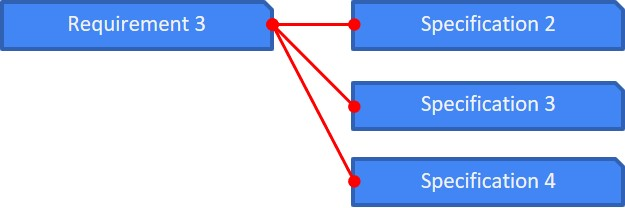
\includegraphics[]{OneToMany.jpg}
    \caption{1 requirement covered by 3 specifications}
    \label{fig:OneToMany}
\end{figure}

So we see here that the complexity of the coverage between requirements and specifications can quickly increase. Just like a spaghetti dish!

\begin{figure}[h]
    \centering
    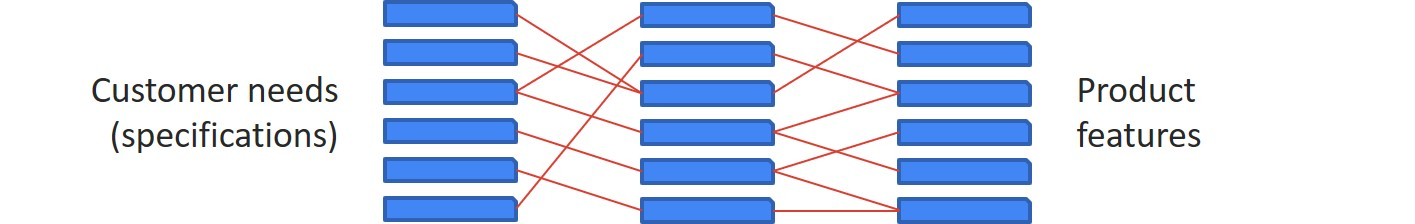
\includegraphics[]{traceability}
    \caption{Many requirements entangled to many specifications}
    \label{fig:WholeTraceability}
\end{figure}

\section{Ok but how exactly?}
\subsection{The structure}
A traceability matrix is an two-columns table where are exhaustively listed every coverage link between every requirements and every specifications. Our previous example would give the following matrix:

\begin{table*}
	\centering
		\begin{tabular}{|c|c|}
			\hline
			\textbf{Customer Requirements} & \textbf{Supplier Specifications}\\
            \hline
            Customer requirement 1 & Supplier specification 1\\
            \hline
            Customer requirement 2 & Supplier specification 1\\
            \hline
            Customer requirement 3 & Supplier specification 2\\
            &Supplier specification3\\
            &Supplier specification 4\\
            \hline
		\end{tabular}
	\caption{Downstream Traceability Matrix}
	\label{tab:DownstreamTraceabilityMatrix}
\end{table*}

On the left, there is the list of the customer’s requirements in the same order they appear in the RFQ. There are given by their title only (or their ID) to avoid an overloaded table.
On the right, for each requirement, the list of the covering customer specifications.

It is very important that on the left column, each requirement appears once and only once. The purpose here is to ensure every requirement is covered by at least one specification.
On the contrary, on the right column, we observe the supplier’s specification 1 is listed twice. This is absolutely normal as this specification matches both customer requirement 1 and customer requirement 2.

\subsection{The point of view and coverage quality}
We can say this matrix adopts the customer’s point of view. It goes from the RFQ to the specifications, that is why it is called the \textbf{Downstream Traceability Matrix}. Once completed, we know exactly the coverage of the customer need. And if one requirement as no specification match, we know the specification document isn’t complete.

But be careful as the devil always hides in the details! The traceability matrix can only tell if a requirement is covered by a specification. I cannot tell if this specification IS ENOUGH to cover the requirement.
Let’s consider again the customer requirement 3. We see it is covered by the following specifications:

\begin{itemize}
    \item Supplier specification 2
    \item Supplier specification 3
    \item Supplier specification 4
\end{itemize}

For example, if the supplier specification 4 is omitted, from the matrix point of view, the customer requirement is still covered. But in reality, without the specification 4, the product wouldn’t match the need.

\section{The other traceability matrices}
We can change the point of view of the matrix to observe the project’s traceability from another angle to ease its management.

\subsection{Upstream Traceability Matrix}
We saw the customer’s point of view with the downstream traceability matrix. Let’s check the supplier’s with the Upstream Traceability Matrix.

\begin{table*}
	\centering
		\begin{tabular}{|c|c|}
			\hline
			\textbf{Supplier Specifications} & \textbf{Customer Requirements}\\
            \hline
            Supplier specification 1 & Customer requirement 1\\
            & Customer requirement 2\\
            \hline
            Supplier specification 2 & Customer requirement 3\\
            \hline
            Supplier specification 3 & Customer requirement 3\\
            \hline
            Supplier specification 4 & Customer requirement 3\\
            \hline
		\end{tabular}
	\caption{Upstream Traceability Matrix}
	\label{tab:UpstreamTraceabilityMatrix}
\end{table*}

On the left, we list the supplier’s specifications in the order they appear in the specification document delivered to the customer, avoiding making duplicates.
On the right, facing each specification, we list all the requirements it covers. This time, it is OK if there are duplicated requirements. It tells that one requirement is covered by several specifications, proving the supplier’s solution is strong and relevant.

This point of view shows if all the specifications cover the requirements and how many requirement are covered by each specification (we will see that sometimes a specification covers nothing)

So in the project’s roadmap, specifications covering the highest number of requirements can be prioritized. In our example, it can be strategic to develop supplier specification 1 to rapidly cover several requirements. Consequently, we can faster reach the minimum valuable product to show the customer. Then we iterate upon it by adding more and more features (aka specifications).

\subsection{Non-covering specification matrix}
It happens that the supplier designs additional specifications covering no requirement. Strange isn’t it?!

Not necessarily. Those orphan specifications may describe constraints for the supplier independent from the customer’s need. But the supplier want to mention them on the specification document to share them with its customer.

For example, the supplier is used to a software, he can tell his customer he will use it through a specification. So that specification will be mandatory without covering any need.
Or the supplier has a special discount for specific components, so he tells thought a specification that he will use this brand over another.
Last example: reading the RFQ, the supplier identifies a hidden need that doesn’t appear in the customer’s requirements. He can add it in his specifications.

He could put those orphan specifications in the upstream matrix, but they would face no requirement. That could bring doubt upon the document: is it a mistake? Is it normal?

To avoid those questioning, the best is to create a new table listing only those non-covering specifications.

% TODO : faire en sorte que le tableau n'apparaisse pas collé au précédent. Une histoire de flottant je crois.
\begin{table*}
	\centering
		\begin{tabular}{|c|}
			\hline
			\textbf{Non-covering specification matrix}\\
            \hline
            Supplier specification 5\\
            \hline
            Supplier specification 6\\
            \hline
            Supplier specification 7\\
            \hline
		\end{tabular}
	\caption{Non-covering Specification Matrix}
	\label{tab:NonCoveringSpecificationMatrix}
\end{table*}

\subsection{Evolution}
It is inevitable! Whether the RFQ or the specification document are intended to evolve. Because the need is more mature, because of the discussions and new ideas come out or bring corrections…

In the document revision 2, some requirements have been updated. But not all of them. So what? Should we read the whole document again? The 200 pages? To only find 3 or 4 modifications?! No! Because there is an evolution matrix!

This matrix doesn’t connect two different documents, it links two revisions of the same document! For example, let’s imagine the RFQ has had 3 modifications as follow:

\begin{table*}
	\centering
		\begin{tabular}{|c|c|}
			\hline
			\textbf{Evolutions} & \textbf{Comments}\\
            \hline
            Customer requirement 2 & Deleted\\
            \hline
            Customer requirement 3.2 & Updated\\
            \hline
            Customer requirement 4 & New\\
            \hline
		\end{tabular}
	\caption{Evolution Matrix}
	\label{tab:EvolutionMatrix}
\end{table*}

\subsection{A deletion}

\begin{table*}
	\centering
		\begin{tabular}{|c|c|}
			\hline
			\textbf{Evolutions} & \textbf{Comments}\\
            \hline
            Customer requirement 2 & Deleted\\
            \hline
		\end{tabular}
	\caption{A deletion}
	\label{tab:Deletion}
\end{table*}

The customer has simply deleted a requirement. It was no longer required or what it described was non longer needed. A deletion in a 200 pages document might be missed. But its impact on the project might be huge because all the specifications that used to cover it are no longer needed either. Therefore they have to be deleted too to avoid useless costs. Besides the planning may be updated too!

I highly advise to keep this deleted requirement in the downstream matrix. But instead of keeping the covering specification, replace them with the comment “deleted” in the specification column. It might be redundant but at least it won’t be forgotten.

\begin{table*}
	\centering
		\begin{tabular}{|c|c|}
			\hline
			\textbf{Customer Requirements} & \textbf{Supplier Specifications}\\
            \hline
            Customer requirement 1 & Supplier specification 1\\
            \hline
            Customer requirement 2 & Deleted\\
            \hline
            Customer requirement 3 & Supplier specification 2\\
            &Supplier specification3\\
            &Supplier specification 4\\
            \hline
		\end{tabular}
	\caption{Downstream Traceability Matrix with a deleted requirement}
	\label{tab:DownstreamTraceabilityMatrixWithDeletedReq}
\end{table*}

\subsection{An update}

\begin{table}
	\centering
		\begin{tabular}{|c|c|}
			\hline
			\textbf{Evolutions} & \textbf{Comments}\\
            \hline
            Customer requirement 3.1 & Updated\\
            \hline
		\end{tabular}
	\caption{An update}
	\label{tab:Update}
\end{table}

A previously existing requirement has been updated. It shall be highlighted because this evolution might have an impact on all the specifications that used to cover the previous revision of this requirement.

We can add a revision number to the requirement’s ID to show its level of update : “Customer requirement 3\textbf{.2}“.

Besides, this would be a good practice to add this revision number to all the requirements. By convention, the original revision of a requirement would be the number 1 : “Customer requirement X\textbf{.1}” (You can choose .0 as the number of the first iteration. It doesn’t really matter, as long as you stick to your convention through the project).

\begin{table}
	\centering
		\begin{tabular}{|c|c|}
			\hline
			\textbf{Customer Requirements} & \textbf{Supplier Specifications}\\
            \hline
            Customer requirement 1.1 & Supplier specification 1.1\\
            \hline
            Customer requirement 2.1 & Deleted\\
            \hline
            Customer requirement 3.2 & Supplier specification 2.2\\
            &Supplier specification 3.2\\
            &Supplier specification 4.2\\
            \hline
		\end{tabular}
	\caption{Downstream traceability matrix with an updated requirement (we observe here that the covering specifications have been updated too for the specification document to be relevant)}
	\label{tab:DownstreamTraceabilityMatrixWithUpdatedReq}
\end{table}

\subsection{A new one}

\begin{table}
	\centering
		\begin{tabular}{|c|c|}
			\hline
			\textbf{Evolutions} & \textbf{Comments}\\
            \hline
            Customer requirement 3.1 & Updated\\
            \hline
		\end{tabular}
	\caption{A new requirement}
	\label{tab:New}
\end{table}

The customer has added a new requirement to detail his need. Just like the other evolutions, without further indication a new requirement can be missed in a 200 hundred page document. Because a new requirement imply the definition of new specifications, its creation shall appear in the evolution matrix, otherwise you may fall through the net. Or as we say in french you get a “trou dans la raquette” (a hole in the racket).

\begin{table}
	\centering
		\begin{tabular}{|c|c|}
			\hline
			\textbf{Customer Requirements} & \textbf{Supplier Specifications}\\
            \hline
            Customer requirement 1.1 & Supplier specification 1.1\\
            \hline
            Customer requirement 2.1 & Deleted\\
            \hline
            Customer requirement 3.2 & Supplier specification 2.2\\
            &Supplier specification 3.2\\
            &Supplier specification 4.2\\
            \hline
            Customer requirement 4.1 & Supplier specification 5.1\\
            \hline
		\end{tabular}
	\caption{Downstream traceability matrix with a new requirement (4.1) which has been immediately covered by a new specification (5.1)}
	\label{tab:DownstreamTraceabilityMatrixWithNewReq}
\end{table}

Long story short, any evolution described in the evolution matrix can, and shall, be also described in the other traceability matrices. It will produce duplicated information but allows you to double-check the consistency of your documents. If you find a loss going from one to another, then there might be a bug in the project. If there isn’t, then you have a very clear view on the project’s management.

\subsection{Ok but what if there is a third revision of the document?}
We still talk about the evolution matrix between two revisions of the same document. First of all, it is totally fine to have a third, a fourth, etc revision of a document. Documentation is a living entity, the blueprint of your project. On some projects, I have already had up to seven revisions for the same document, it’s usual business.

So if you have a third revision (v3) then you should make an evolution matrix showing the updates between v2 and v3.

It is not mandatory, but it can be helpful to keep all the evolution matrices in every new revision. Like this, you’ll have a complete historic of your document without having to open all the previous revisions to have the big picture. But beware, in the end, it might be a lot of matrices!

\section{The Fantastic Matrices and where to find them}
Let’s draw another table to explain where and how to draw those matrices:

\begin{table}
	\centering
		\begin{tabular}{|c|c|c|c|c|c|}
			\hline
			\textbf{Matrices} & \textbf{v1} & \textbf{v2} & \textbf{v3} & \textbf{...} & \textbf{vN}\\
            & \textbf{Original document}& & & & \\
            \hline
            \textbf{D}ownstream & $D_1$ & $D_2$ & $D_3$ & ... & $D_N$ \\
            &compliant with $U_1$ and $NC_1$ &&&&\\
            \hline
            \textbf{U}pstream& $U_1$ & $U_2$ & $U_3$ & ... & $U_N$ \\
            &compliant with $D_1$ and $NC_1$ &&&&\\
            \hline
            \textbf{N}on \textbf{C}overing& $NC_1$ & $NC_2$ & $NC_3$ & ... & $NC_N$ \\
            &compliant with $D_1$ and $U_1$ &&&&\\
            \hline
            \textbf{E}volution& At this point there is & $E_{1 \to 2}$ & $E_{2 \to 3}$ &...& \[ \sum_{n=2}^{N} $E_{n-1 \to n}$ \] \\
            &no evolution matrix&Evolutions from v1 to v2&+ $E_{1 \to 2}$&&\\
            \hline
		\end{tabular}
	\caption{Matrices to add to your document depending on its revision}
	\label{tab:MatricesMatrix}
\end{table}

\section{Conclusion}
The traceability matrix is a very powerful tool! It provides an exhaustive view on the customer’s need’s coverage; ensures that nothing is forgotten and allows the project to be customer’s-evolution-proof and makes it resilient.

But what if I told you we only scratched the surface ?

Indeed, we considered the links between the customer’s requirements and the supplier’s specifications. But in the process of a project, this is just the first step. Then more detailed specifications can be written (functional specifications for example) then design document, validation plan, etc. All of them are connected and the links between all those documents shall be tracked too for the same reasons.

But no more drama. The concepts presented here are relevant for all the links. Some of them may require some adjustments. We may have some slightly different matrices for them. But let’s stop here for the moment.

The more complex or the bigger a project is, the more documents it has. It will require more and more strictness to build the matrices without forgetting anything and ensure the customer’s need is 100\% covered. Among other issues, building trusted matrices and getting a consistent documentation is why we created Naept which does it automatically (and so much more!).
